\subsubsection{Task hinzufügen (Applikation)}

\begin{figure}[H]
    \begin{center}
      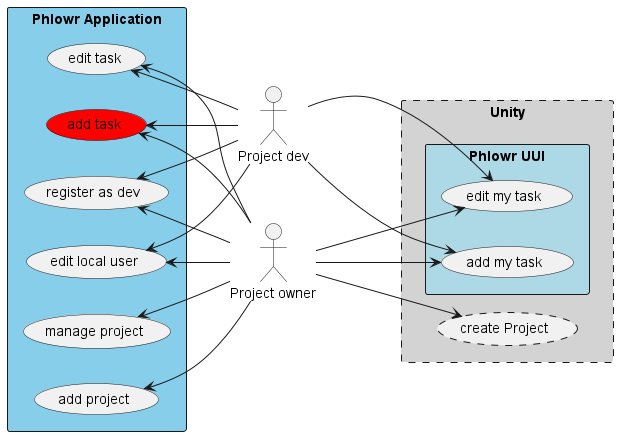
\includegraphics[width=0.25\linewidth]{../content/diagrams/usecase/overview/overviewUseCaseAddTaskSelected.png}
      \caption{Use Case Diagaramm <add Task> }
    \end{center}
  \end{figure}

  \begin{table}[H]
    \centering
    \settowidth\tymin{executeIncomingCommand()}
    \setlength\extrarowheight{2pt}
    \begin{tabulary}{1.0\textwidth}{|m{4cm}|m{9cm}|}
      \hline
      \textbf{Use Case} &
      \textbf{ADD TASK}\\
      \hline
      \textbf{Beschreibung} &
      Ein Task wird dem Projekt hinzugefügt\\ 
      \hline
      \textbf{Includes} &
      \begin{itemize}
       \item keine
        \end{itemize}\\ 
        \hline 
      \textbf{Akteure} &
      \begin{itemize}
       \item Entwickler
       \item Projekt-Owner
        \end{itemize}\\  
        \hline
      \textbf{Auslöser} &
      \begin{itemize}
        \item Ein Task soll dem Projekt hinzugefügt werden
         \end{itemize}\\  
      \hline
      \textbf{Vorbedingungen} &
      \begin{itemize}
        \item Das Projekt ist der Applikation hinzugefügt
        \item Der Ersteller ist Projekt-Owner oder beim Projekt als Entwickler registriert
        \item das Projekt ist auf dem aktuellsten Stand
      \end{itemize}\\  
      \hline
      \textbf{Abschlussbedingunen} &
      Ein neuer Task ist im Projekt verfügbar\\
      \hline
      \textbf{Ablauf} &
      \begin{enumerate}
        \item Applikation öffnen
        \item Projekt öffnen
        \item <Task hinzufügen> klicken
        \item Details des neuen Tasks ausfüllen (Name, Beschreibung usw.)
        \item Speichern
        \item Projekt synchronisieren
        \end{enumerate}\\ 
      \hline
      \textbf{Zu Beachten / Notizen} &
      \begin{itemize}
        \item Tasks können ebenfalls bei bereits existierenden Tasks hinzugefügt werden, dazu wird einfach der entsprechende Task geöffnet.
        \end{itemize}\\ 
      \hline
    \end{tabulary}
    \caption{Use Case: add task}
  \end{table}
 